\problemname{Armstöd}

Petitess-organisationen (PO) har möte och de $N$ medlemmarna sitter på
stolar i en ring, vända inåt. Mellan varje par av stolar finns ett armstöd som högst en av personerna kan använda. Varje person har en preferens i form av vilken eller vilka armar hen vill placera på armstöden:
\begin{itemize}
\item V: vänster arm
\item H: höger arm
\item A: antingen vänster eller höger arm
\item B: båda armarna
\item I: ingen arm
\end{itemize}

Skriv ett program som beräknar hur många av personerna som maximalt kan bli nöjda.

\section*{Indata}
På första raden står ett heltal $N$, antal personer i ringen. På andra raden står personernas preferenser, givna i den ordning
personerna sitter, {\em moturs} i ringen, i form av en
sträng bestående av $N$ bokstäver, vardera \texttt{V}, \texttt{H},
\texttt{A}, \texttt{B} eller \texttt{I}. 

\section*{Utdata}
Programmet ska skriva ut ett heltal: det maximala antalet personer som kan få sin preferens uppfylld.

\begin{figure}[!htb]
\begin{center}
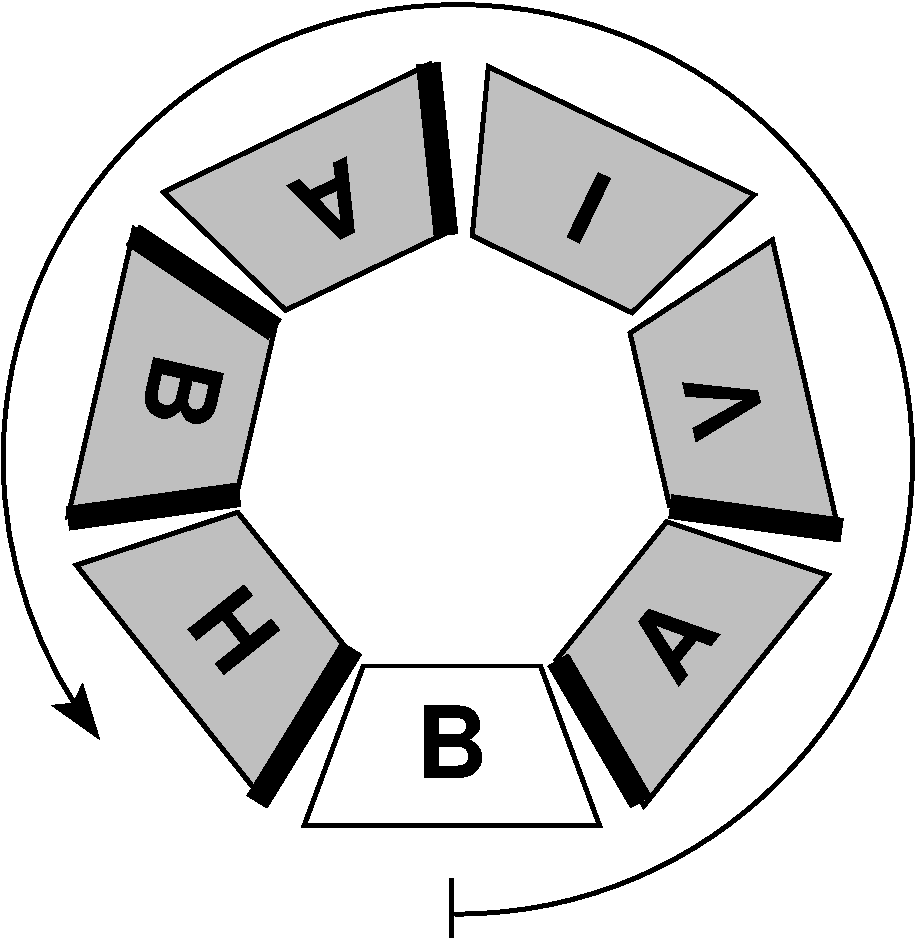
\includegraphics[width=5cm]{armstodbild.pdf}
\end{center}
\caption{Figuren visar lösningen till exempel 1. De tjocka linjerna markerar
armar som personer lagt på armstöden. Den grå färgen visar vilka som fått sina preferenser uppfyllda. Pilen markerar var den givna
indatasträngen börjar och slutar.}
\end{figure}

\section*{Poängsättning}

För testfall värda 
\begin{tabular}{llll}
$20$ poäng & gäller att &N=5$ & och första bokstaven är I. \\
$40$ poäng &  & $6\le N\le 15$ &, vilka bokstäver som helst.\\
$20$ poäng &  & $25\le N\le 30$ & och första bokstaven är I. \\
$20$ poäng &  & $25\le N\le 30$ &, vilka bokstäver som helst. \\
\end{tabular}                          
